%! Author = a
%! Date = 12/5/24

After the successful training of pathfinder, we switched to a harder task: designing the collider.
We decided to use trained pathfinder as the target for collider.

\subsection{Objective}\label{subsec:collider_objective}
Collider should intercept the pathfinder before it has reached the destination.

\subsection{Observations}\label{subsec:collider_observations}
During the tests, we figured out that pathfinder is able to reach even moving target.
However, we decided to include the target velocities to colliders observations among with pathfinder's observations.
So, the final vector would include:
\begin{itemize}
	\item Target relative position
	\item Target linear velocity
	\item Target angular velocity
	\item Agent linear velocity
	\item Agent angular velocity
	\item Agent front, right and up vectors
\end{itemize}
We didn't include the pathfinder's target in observations,
as the collider could potentially learn the pathfinder's behavior.

\subsection{Actions}\label{subsec:collider_actions}
The set of actions for collider is the same as for pathfinder.

\subsection{Reward}\label{subsec:reward}
Pathfinder's simple reward didn't work in the collider case,
as the chance of randomly hitting the target was significantly lower.
That's why the designed reward function had to guide the agent in the right direction.
However, the reward should not be extremely strict.
Penalizing the agent for not following some strictly defined route would force agent learning that route.

\subsubsection{Negative distance}
The initial idea was to use the distance to the target as a reward function.
The agent would be penalized for being far from the target more than getting closer:
\[
	-\left|\vec{p_t} - \vec{p_a}\right|
\] where
\begin{itemize}
	\item $\vec{p_t}$ is the target position
	\item $\vec{p_a}$ is the agent position
\end{itemize}

We could also use inverse distance ${\left|\vec{p_t} - \vec{p_a}\right|^{-1}}$.
However, the positive reward from keeping close to the object has to be balanced with negative reward for the episode duration.
Otherwise, the agent will circle around the target but not reaching it, increasing its reward infinitely.

Surprisingly, this reward didn't give us reliable results.
So, we moved to velocity projection policy.

\subsubsection{Velocity projection}
This reward was designed to hint the correct direction for the agent.
Simply projection the linear velocity vector magnitude onto the vector to the target, we will get positive values for heading to the target and negative for going away:
\[
	\frac{\vec{v_a} \cdot (\vec{p_t} - \vec{p_a})}{\left|\vec{p_t} - \vec{p_a}\right|}
\] where
\begin{itemize}
	\item $\vec{p_t}$ is the target position
	\item $\vec{p_a}$ is the agent position
\end{itemize}

Agent trained with this reward was able to follow the direct path to the target.
However, the collider was always followed behind the pathfinder, instead of trying to intercept it.
This led to the development of a rendezvous distance.

\subsubsection{Rendezvous distance}
The idea behind this reward is to minimize the distance between the closest points in the future.
Position along the axis $n$ can be easily predicted given the velocity function along this axis $v_n(t)$:
\[
	p_n(T) = \int_{0}^{T}v_n(t)dt
\]
Given initial position $P_n$, constant velocity $v_n$ and acceleration $a_n$, this leads to:
\[
	p_n(t) = P_n + t v_n + \frac{t^2}{2} a_n
\]
So, the distance between two objects $x$ and $y$ in $N$-dimensional space can be defined as:
\[
	f(t) = \sum_{n=1}^{N} \left(p_n^x(t) - p_n^y(t)\right)^2
\]
We can find the moment $T$ when the distance is going to be minimal, checking extreme points of this function.
To find the extreme points we need to find solutions to:
\begin{gather*}
	\odv{f(t)}{t} = 0 \\
	\odv{f(t)}{t} = 2 \sum_{n=1}^{N}(\Delta P_n + t \Delta v_n + \frac{t^2}{2} \Delta a_n)(\Delta v_n + t \Delta a_n)
\end{gather*}
\begin{align*}
	\intertext{where}
	\Delta P_n &= P_n^x - P_n^y \\
	\Delta v_n &= v_n^x - v_n^y \\
	\Delta a_n &= a_n^x - a_n^y \\
	\intertext{It can be rewritten in a more compact form:}
	\odv{f(t)}{t} &= 2(at^3 + bt^2 + ct + d) \\
	\intertext{where}
	a &= \frac{1}{2} \Delta \vec{a} \cdot \Delta \vec{a} \\
	b &= \frac{3}{2} \Delta \vec{a} \cdot \Delta \vec{v} \\
	c &= \Delta \vec{P} \cdot \Delta \vec{a} + \Delta \vec{v} \cdot \Delta \vec{v} \\
	d &= \Delta \vec{P} \cdot \Delta \vec{v}
\end{align*}
Leading to a simple cubic equation:
\[
	2(at^3 + bt^2 + ct + d) = 0
\]
This cubic equation can be solved using modified Cardano's method described in the Numerical Recipes book.
Then checking solutions for $t$ we can find the minimal distance in the future.
The agent will be penalized using this distance as a negative reward.

The demonstration for these calculations is available in Desmos: \url{https://www.desmos.com/calculator/rgrunpbkbd}
\begin{figure}[H]
	\centering
	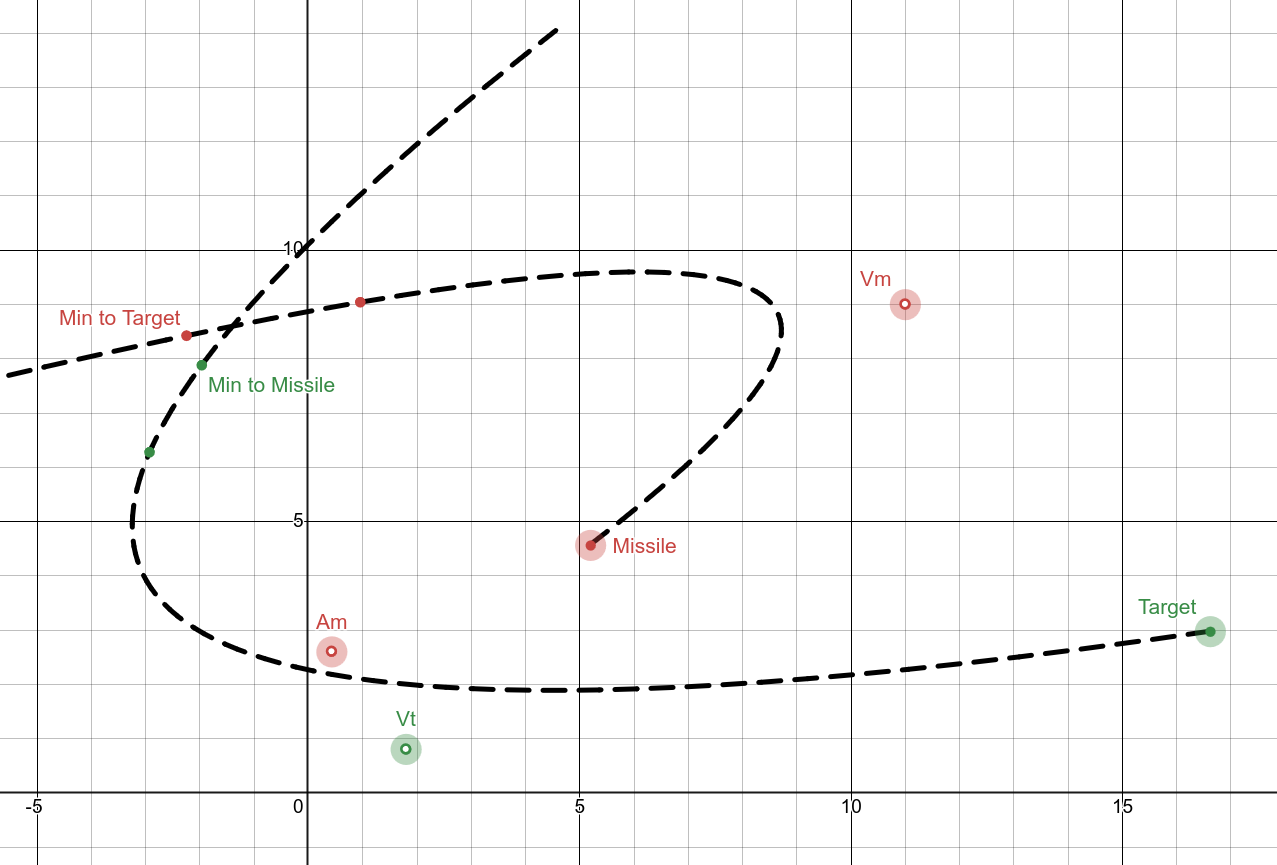
\includegraphics[width=0.5\textwidth]{images/rendezvous.png}
	\caption{Prediction of trajectories and closest points}
	\label{fig:rendezvous}
\end{figure}

However, even this reward couldn't solve the situation.
This was the moment we started to suspect that something was going wrong.